\documentclass{article}
\usepackage{amsmath}
\usepackage{amsfonts}
\usepackage{amssymb}
\usepackage{tcolorbox}
\usepackage[inline]{enumitem}
\usepackage[a4paper,margin=1in]{geometry}
\usepackage[normalem]{ulem}
\usepackage{graphicx}
\usepackage{tasks}
\settasks{label=(\alph*), label-offset=0.4em, label-width=1.5em}

\usepackage{fancyhdr}
\fancyhf{}
\setlength{\headheight}{36pt}
\renewcommand{\headrulewidth}{0pt}
\thispagestyle{fancy}
\lhead{Calculus Exercise}
\chead{Week 11 (6.1, 6.2, 6.3, 6.5)}
\rhead{\underline{ID:\hspace{7.4em}} \\ \vspace{0.2cm} \uline{Name:\hspace{6em}}}
\cfoot{\thepage}

\begin{document}
\begin{enumerate}
\item[6.1.18]
    Sketch the region enclosed by the given curves. Decide whether to integrate with
    respect to $x$ or $y$. Draw a typical approximating rectangle and label its
    height and width. Then find the area of the region.
    \[
        4x+y^{2} = 12,\ x=y
    \]

\vspace{6cm}

\item[6.1.31]
    Sketch the region enclosed by the given curves and find tis area.
    \[
        y = x^{4},\ y = 2 - | x |
    \]

\vspace{6cm}

\item[6.1.42]
    Use calculus to find the area of the triangle with the given vertices:
    $(2, 0),\ (0, 2),\ , (-1, 1)$.

\newpage

\item[6.1.43]
    Evaluate the integral and interpret it as the area of a region. Sketch the
    region.
    \[
        \int_{0}^{\frac{\pi}{2}} | \sin (x) - \cos (2x) | dx
    \]

\vspace{8cm}

\item[6.1.69]
    The figure shows a horizontal line $y=c$ intersecting the curve $y=8x-27x^{3}$.
    Find the number $c$ such that the areas of the shaded regions are equal.

    \begin{center}
        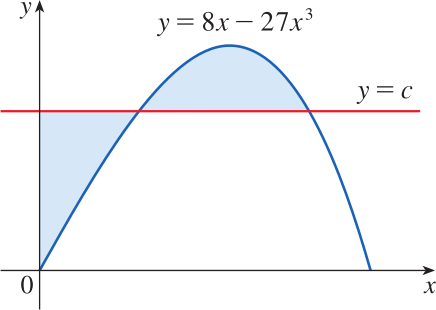
\includegraphics[width=5cm]{./png/6.1.69.png}
    \end{center}

\newpage

\item[6.2.44]
    Set up an integral for the volume of the solid obtained by rotating the
    region bounded by the given curves about the specified line. Then use
    a calculator or computer to evaluate the integral correct to five decimal places.
    \[
        y = x^{2},\ x^{2} + y^{2} = 1,\ y \geqslant 0
    \]
    (a) About the $x$-axis (b) About the $y$-axis

\vspace{8cm}

\item[6.2.62]
    A frustum of a pyramid with square base of side $b$, square top of side $a$,
    and height $h$. What happens if $a=b$? What happens if $a=0$?

    \begin{center}
        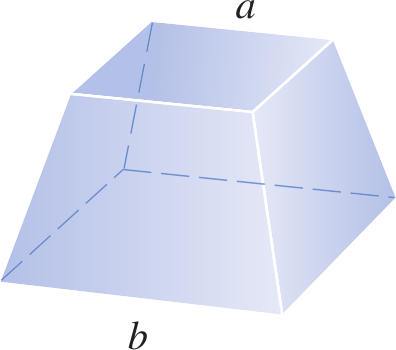
\includegraphics[width=5cm]{./png/6.2.62.png}
    \end{center}

\newpage

\item[6.2.74]
    Cross-sections of the solid $S$ in planes perpendicular to the $x$-axis are
    circles with diameters extending from the curve $y=\frac{1}{2}\sqrt{x}$
    to the curve $y=\sqrt{x}$ for $0 \leqslant x \leqslant 4$.

    \begin{center}
        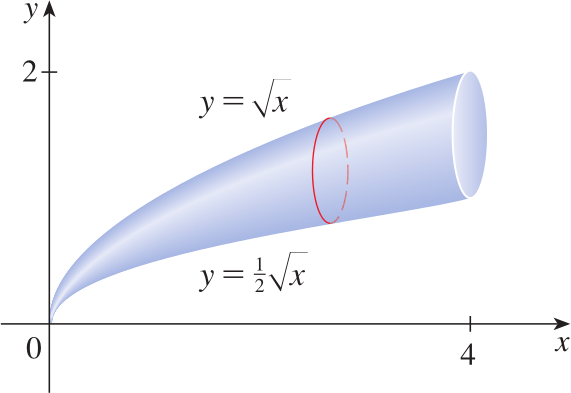
\includegraphics[width=6cm]{./png/6.2.74.png}
    \end{center}

\vspace{6cm}

\item[6.2.86]
    Suppose that a region $R$ has area $A$ and lies above the $x$-axis.
    When $R$ is rotated about the $x$-axis, it sweeps out a solid with
    volume $V_1$. When $R$ is rotated about the line $y=-k$ (where
    $k$ is a positive number), it sweeps out a solid with volume $V_2$.
    Express $V_2$ in terms of $V_1, k$, and $A$.

\newpage

\item[6.3.47]
    A solid is obtained by rotating the shaded region about the $y$-axis.
    \begin{enumerate}
        \item Set up an integral using any method to find the volume of the solid.
        \item Evaluate the integral to find the volume of the solid.
    \end{enumerate}
    \begin{center}
        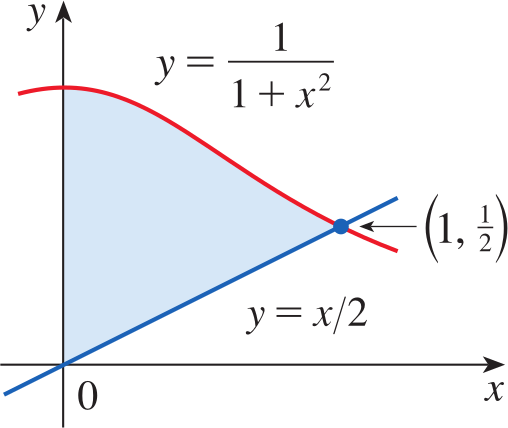
\includegraphics[width=5cm]{./png/6.3.47.png}
    \end{center}

\vspace{6cm}

\item[6.3.55]
    The region bounded by the given curves is rotated about the specified axis.
    Find the volume of the resulting solid by any method.
    \[
        y^{2}-x^{2}=1,\ y=2; \text{ about the $x$-axis }
    \]

\newpage

\item[6.3.56]
    Same as 6.3.55.
    \[
        y^{2}-x^{2}=1,\ y=2; \text{ about the $y$-axis }
    \]

\vspace{5cm}

\item[6.3.62]
    Use cylindrical shells to find the volume of the solid torus.
    \begin{center}
        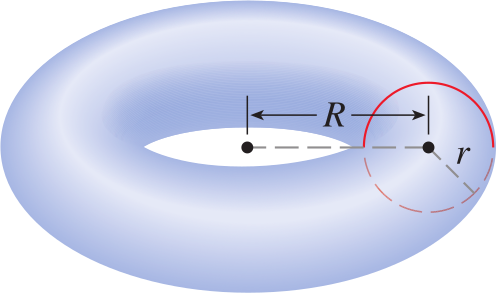
\includegraphics[width=5cm]{./png/6.3.62.png}
    \end{center}

\vspace{5cm}

\item[6.5.13]
    If $f$ is continuous and $\displaystyle \int_{1}^{3} f(x) dx=8$, show
    that $f$ takes on the value $4$ at least once on the interval $[1, 3]$.

\newpage

\item[6.5.25]
    Use the diagram to show that if $f$ is concave upward on $[a, b]$,
    then
    \[
        \frac{1}{b-a} \int_{a}^{b} f(x) dx > f\left( \frac{a+b}{2} \right)
    \]
    \begin{center}
        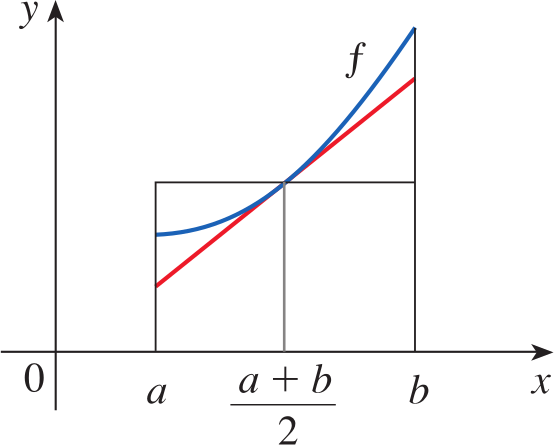
\includegraphics[width=6cm]{./png/6.5.25.png}
    \end{center}

\vspace{6cm}

\item[6.5.26]
    Let $f_{\text{avg}}$ denote the average value of $f$ on the
    interval $[a, b]$. Show that if $a < c < b$, then
    \[
        f_{\text{avg}}[a, b] = \left(\frac{c-a}{b-a}\right) f_{\text{avg}}[a, c]
        + \left( \frac{b-c}{b-a} \right) f_{\text{avg}}[c, b]
    \]

\end{enumerate}
\end{document}
